\section{Strategy}

The main focus was to create an attacking strategy which would utilise the speed of the robot. The strategy was split into two sections, the high level areas (where the robot will move to, when to kick, dribble etc), and the lower level areas (coding the movement of the robot).

\subsection{High Level Strategy}
Initially we created a simple state system strategy, which checked the current on-pitch situation (using the data sent from the camera) and decided the appropriate strategy to run. The state system approach was used because new states could be added easily, allowing for multiple strategies.
Our strategy was based on defining a point to move towards. A point class was created, holding the x,y co-ordinates of points on the pitch. This class was extended to create instances of the robot, ball, goal, and any other necessary points for use in the strategy.


An optimum point was implemented (Algorithm 1), which would be a defined distance behind the ball at the same angle as the ball to goal angle, such that the robot would move to this point, and then to the ball, to ensure the robot was facing the goal when it reached the ball. This worked well in practice, working everytime when the robot was behind the ball, and 9/10 times when the robot was inbetween the goal and the ball (i.e. had to navigate around the ball).

\begin{algorithm}
\caption{Caclulate Optimum Point}
\label{optimumPoint}
\begin{algorithmic}[1]
\STATE $threshold \gets 70$
\STATE $(x_{1}, y_{1}) \gets ball (x, y)$
\STATE $(x_{2}, y_{2}) \gets goal (x, y)$
\STATE $ballGoalAngle = atan2( (y_{2} - y_{1}), (x_{2} - x_{1}) )$
%\STATE $hyp = \sqrt{\alpha^{2} + threshold^{2}}$
%\STATE $\theta = \sin(\frac{100}{hyp})$
\STATE $xOffset = threshold(\cos(ballGoallAngle)$
\STATE $yOffset = threshold(\sin(ballGoalAngle))$
\STATE $(x_{3}, y_{3}) = (x_{1} - xOffset, y_{1} - yOffset)$
\RETURN $(x_{3}, y_{3})$
\end{algorithmic}
\end{algorithm}

This function was later abstracted to a higher level, modifying the function to take any two points and return the angle between them, to increase its range and decrease repetition of similar code. \linebreak

The next target was to be able to navigate around objects. Points were used again, utilised in a function which would calculate an avoidance point at a $90^{\circ}$ angle and a defined distance from the object to avoid. The function would return the avoidance point, and the robot would move to it. \\
This function was dynamic, and the point would move as the robot moved, allowing the robot to navigate the object more smoothly.\\
The function calculated the avoid point using trigonometry, as shown in Algorithm 2 and the following diagram:
\begin{center}
\begin{figure}[htp]
\leavevmode
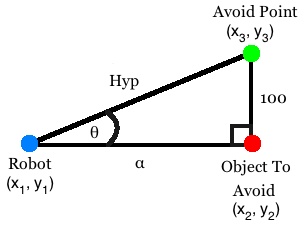
\includegraphics[scale=0.6]{images/AvoidPoints.png}
\label{AvoidPointDiagram}
\end{figure}
\end{center}

\begin{algorithm}
\caption{Caclulate Avoid Point}
\label{avoidPoint}
\begin{algorithmic}[1]
\STATE $threshold \gets 100$
\STATE $(x_{1}, y_{1}) \gets Robot (x, y)$
\STATE $(x_{2}, y_{2}) \gets Object To Avoid (x, y)$
\STATE $\alpha = \sqrt{(x_{2} - x_{1})^{2} + (y_{2} - y_{1})^{2}}$
\STATE $hyp = \sqrt{\alpha^{2} + threshold^{2}}$
\STATE $\theta = \sin(\frac{100}{hyp})$
\STATE $xOffset = hyp(\cos\theta)$
\STATE $yOffset = hyp(\sin\theta)$
\STATE $(x_{3}, y_{3}) = (x_{1} + xOffset, y_{1} + yOffset)$
\RETURN $(x_{3}, y_{3})$
\end{algorithmic}
\end{algorithm}

Again, this function was abstracted to a higher level to calculate the avoidance point for any object, as the robot may need to avoid a ball or a robot, which was useful for the function created to avoid the ball when moving the robot to get to the correct side of the ball (so the ball would be between the robot and the goal we were attacking). \linebreak

Getting the ball away from the wall proved to be problem in our friendly matches as our robot could not reach the optimum point due to it being off the pitch. To counteract this, a strategy was developed to kick the ball towards the wall in the direction of the opponent's goal. Figure \ref{fig:rebound} shows the required rebound point, the equations below give x,y coordinates of rebound point.
\[y = \left\{ 
\begin{array}{l l}
  0 & \quad \mbox{ballY $<$ 155}\\
  310 & \quad \mbox{otherwise}\\ \end{array} \right. \]
\[x = \frac{ballX(goalY-y) + goalX(ballY-y)}{ballY + goalY - 2y} \]
In solving these equations the angle of entry and exit of the ball are assumed to be equal. This assumption worked perfectly when testing the strategy on the simulator however, through tests on the pitch, if the ball had lost speed before hitting the wall the rebound angle was dramatically reduced and the ball remained close to the wall. 

To ensure the ball the ball approached the wall with enough speed, the GetBallFromWall strategy was only ever activated when the ball was 30 pixels\footnote{All distances were measured as pixels based on images captured from the video feed} away from the wall. Adjusting the equations to be more precise is very hard as it would require taking into consideration the spin of the ball, frictional coefficients of both objects and the coefficient of restitution. The simple model proved effective at getting the ball back into open play and occasionally scored a goal.\linebreak

Alongside these additions, functions were implemented which decided if the ball was in more difficult positions, such as being close to the walls or in the corners, for use in the state system, so different strategies could be brought in to deal with these situations. The strategies were further adapted to readjust to a change in the goal we were attacking. 

A more precise shooting system (i.e. being able to shoot directly into the corners of the goal) and a defensive strategy would have improved our performance in the final competition, as a number of shots were saved in the centre of the goal, and we had no real strategy to deal with the opponent having possession, and whilst usually the attacking strategy would cover most defensive situations, we were found out once or twice in the final game. Other than these faults, the strategies worked successfully, and made good use of the robots speed.

\subsection{Low Level Motion}
In low level motion planning layer of the agent architecture we needed a robust algorithm capable of compensating possible noise incurred by output of vision stack.  The simple goal for this part is to make robot capable of following a path to reach a destination position determined by higher levels of path planning algorithm.\linebreak

\subsubsection{Potential Field}
To achieve the goal stated above we started with implementing Potential Fields\cite{paper:PF} algorithm. This algorithm is a well-known method for robot path planning. It has several properties which makes it suitable for our application. The behaviour of the algorithm is completely reactive and therefore if it is fed with noisy input in one cycle it will be able to recover in next cycles, therefore performance of the algorithm degrades as amount of noise increases never failing completely.\linebreak

\subsubsection{Challenges}
During implementation of this method, we had several challenges. We started testing this algorithm for milestone two but failed. The initial intuition for most members was that the failure was due to complexity of this algorithm while the failure was in fact due to unreliable input produced by vision stack. Later, new set of tests showed a very good performance once the vision stack become robust and reliable. Successful implementation of this algorithm was a key to our success in third and fourth friendly matches.\linebreak

\subsubsection{Kinematic Model and Implementation}
In order to implement this algorithm successfully we needed to find a way to apply the calculated velocity vector from previous step on the robot. To do this, we used a kinematic model of a differential drive robot. In figure \ref{KinModel},the velocity vector is decomposed into linear and angular velocity and later they are fused to calculate velocity of left and right wheels.
\begin{figure}[htp]
\begin{center}
\leavevmode
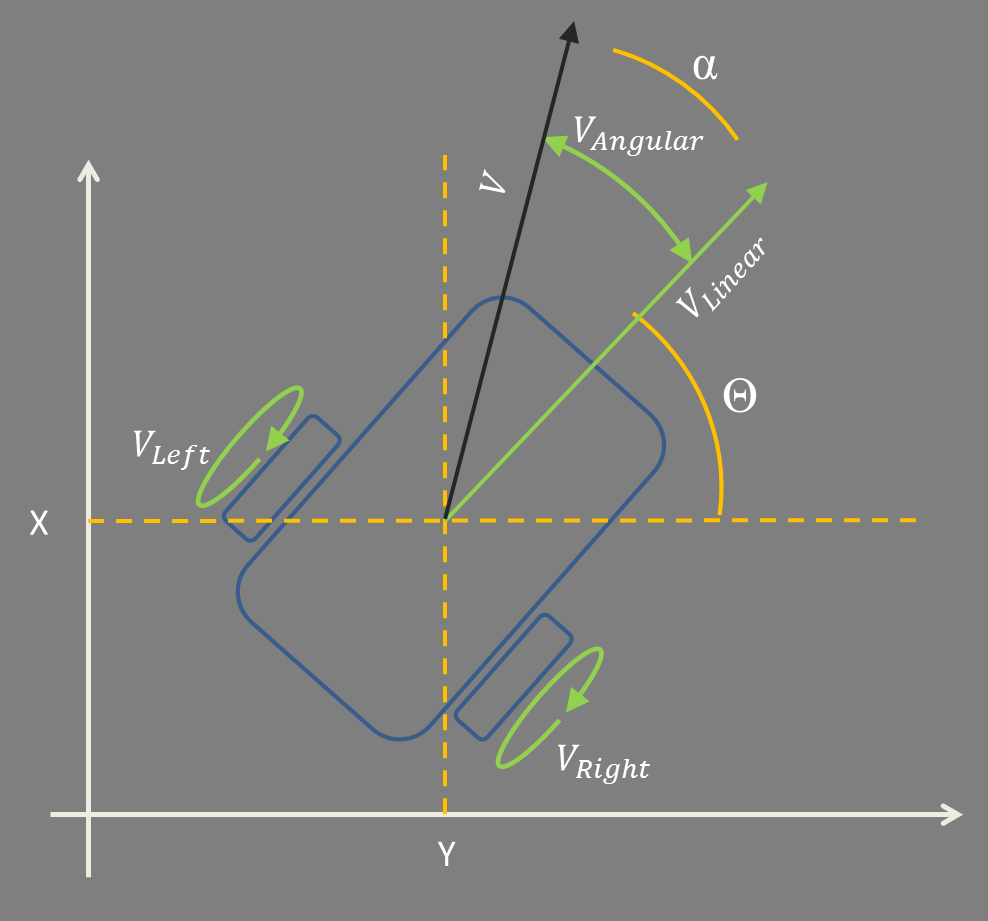
\includegraphics[width=0.25\textwidth] {KinModel.png}
\end{center}
\caption{Kinematic Model of Non-holonomic Differential Drive Robot}
\label{fig:KinModel}
\end{figure}
\begin{align}
V & =k_{att}.(Pos_{current}-Pos_{destination})\\
V_{linear} &= \begin{Vmatrix}v\end{Vmatrix} cos(\theta) ,
V_{angular} = {K\theta \over \pi}\\
V_{left}&=V_{Linear}-rsin(V_{Angular})\\
V_{right}&=V_{Linear}+rsin(V_{Angular})
\end{align}

Integrating all this we were able to implement a successful motion planning algorithm which distinguished our team from other teams.\linebreak

\subsubsection{Results}
A sample result of running this algorithm on the pitch is demonstrated in figure \ref{fig:seq}, Overall, this algorithm could deal with almost all scenarios successfully and when integrated with a high level decision making layer, we had a reliable game play scenario. 
The solution also can also deal effectively with obstacles using Extended Potential Field algorithm\cite{paper:OKhatib} but this feature was not used because obstacle avoidance was dealt with by higher levels of decision making. Therefore, the algorithm at this level is a conventional P controller.  

\begin{figure}[!bp]
\begin{center}
\subfigure[]{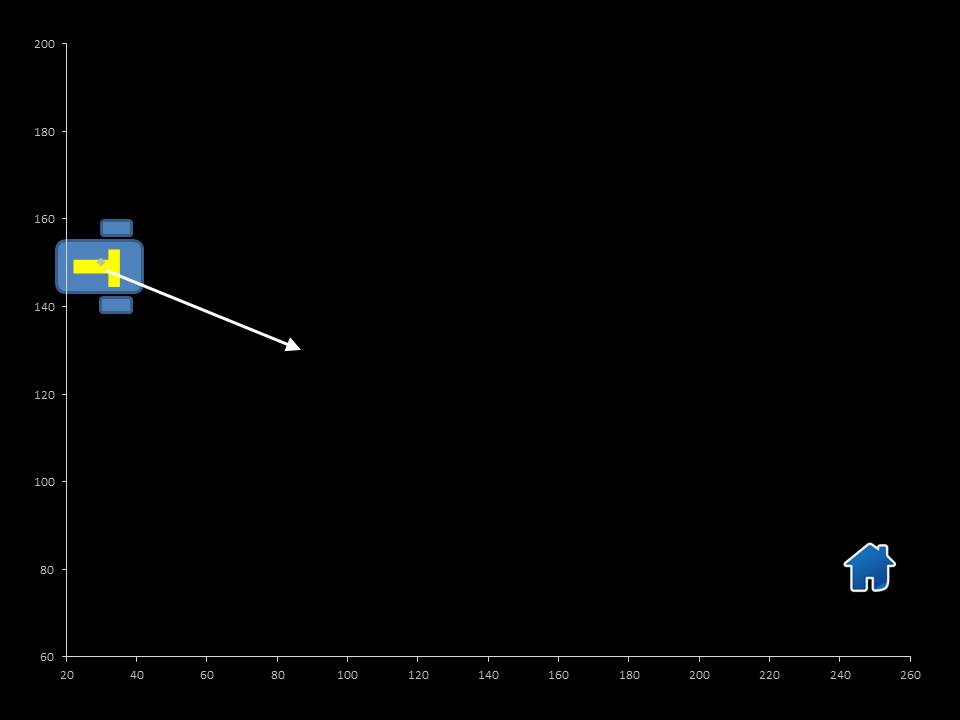
\includegraphics[width=0.15\textwidth] {step1.jpg}}
\subfigure[]{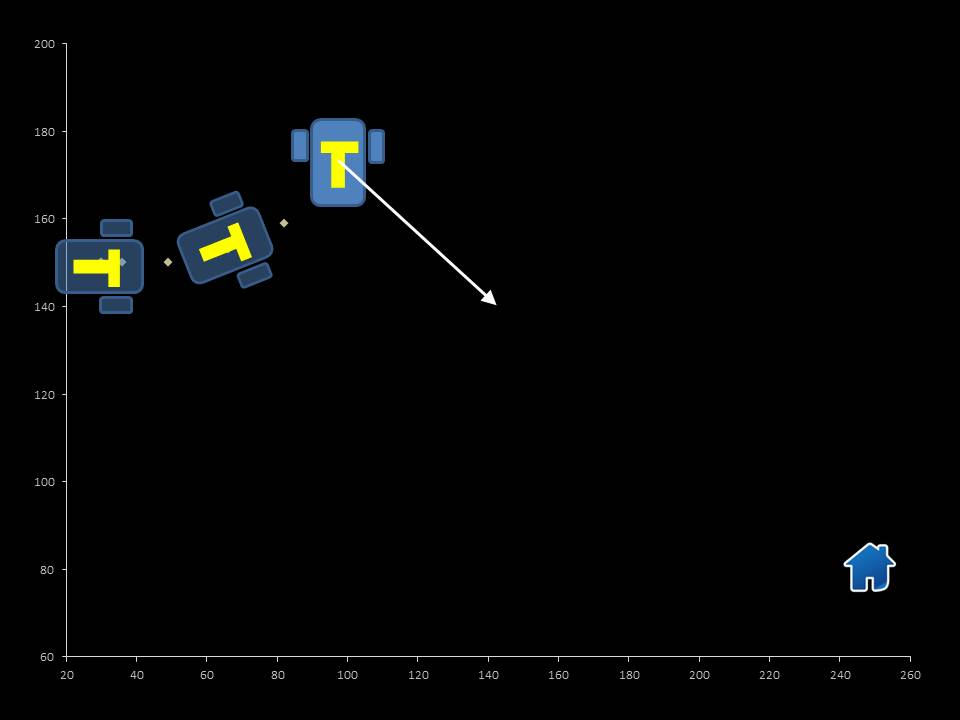
\includegraphics[width=0.15\textwidth] {step2.jpg}}
\subfigure[]{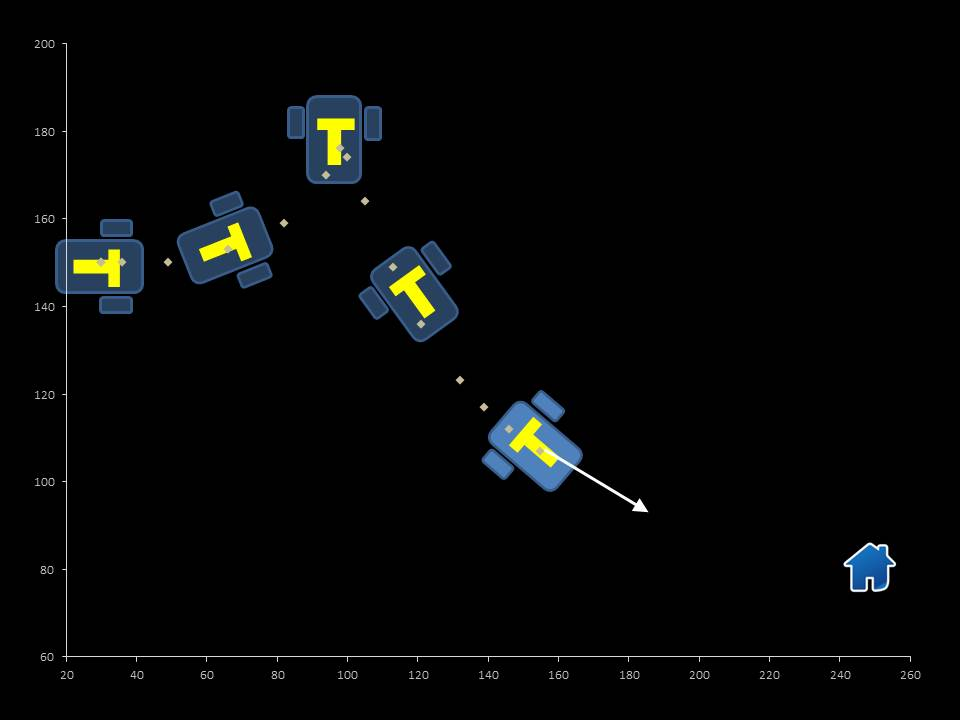
\includegraphics[width=0.15\textwidth] {step3.jpg}}
\subfigure[]{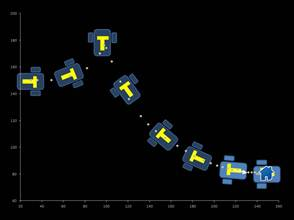
\includegraphics[width=0.15\textwidth] {Final.jpg}}
\caption{A sequence of robot movements from start position to destination.}
\label{fig:seq}
\end{center}
\end{figure}

\subsubsection{Lessons Learned}

\begin{itemize}
\item It is possible to implement reliable applications based on ideas developed in research labs. 
\item Failure of an algorithm at higher levels sometimes may be due to invalid inputs from lower layers.
\item Simulation at abstract level is very useful for making sure that an algorithm is developed according to specification but successful implementation based on such simulation environments does does not guarantee optimal performance in real environments.
\end{itemize}